%!TEX root = ../template.tex
%%%%%%%%%%%%%%%%%%%%%%%%%%%%%%%%%%%%%%%%%%%%%%%%%%%%%%%%%%%%%%%%%%%%
%% chapter2.tex
%% NOVA thesis document file
%%
%% Chapter with the template manual
%%%%%%%%%%%%%%%%%%%%%%%%%%%%%%%%%%%%%%%%%%%%%%%%%%%%%%%%%%%%%%%%%%%%
\chapter{Related Work}
\label{cha:related_work}

% ================
% = Introduction =
% ================
We’re currently in a period where we start to depend more and more on allowing remote services to access our data and execute our applications. Cloud computing systems require users to trust them with their data. Therefore these systems need a way to assure data privacy
and security, thus gaining users trust.

In this chapter we address existing solutions that are able to protect applications from the \gls{os} or hypervisor, regardless the machine where they're running on, thus increasing the level of trust an user can deposit in an execution of an application.

These existing solutions are organized in different sections in the following way: 
Section 2.1 covers protection against untrusted \gls{os}es; 
Section 2.2 covers \gls{tee}s and hardware-enabled approaches;
In Section 2.3 we cover, in more detail, hardware-enabled \gls{tee} solutions used today.
Section 2.4 covers shielded applications and frameworks compatible with Intel-\gls{sgx}, which is the \gls{tee} technology we choose for our approach.
Finally, in Section 2.5 we make a critical analysis on the topics previously discussed, while covering their main advantages and disadvantages.


% =======================
%  N E W   S E C T I O N        (2.1)
% =======================


\section{Protection in untrusted OSes}

A lot of applications these days depend on sensitive data to operate. Therefore protecting this data must be taken into account while designing the application. 
One of the things we have to think about is the size of the \gls{tcb}, and how to reduce it as much as possible without losing the operability of the system. 
Typically, the host \gls{os} is considered safe and trustworthy, although that is not always the case. A compromised \gls{os} can give complete access to sensitive data, if not isolated from the application. That’s why this is a major security problem and must be tackled in today’s systems.

Approaches like Virtual Ghost, Flicker, MUSHI, SeCage, InkTag, Sego, all grant security by isolating the sensitive data from the untrusted \gls{os} either by monitoring the application while it runs, or by enforcing memory isolation by using virtualization.

%-----------------------------------------

Virtual Ghost \cite{virtGhostPaper} provides application security against untrusted \gls{os}es by implementing the idea of ghost memory, which is unaccessible for the \gls{os} to read or write, as well as providing trusted services like ghost memory management, key management, and encryption and signing services. 

It relies in sandboxing to protect the system from the \gls{os}, where a thin layer of abstraction is interposed between the kernel and the hardware. This layer works as a library of functions that the kernel can call directly, without the need of higher priviledges being given to it. 

Thus, Virtual Ghost protects the system against a direct threat from the \gls{os}, without losing significant levels of performance.

%-----------------------------------------

Flicker \cite{flickerPaper} provides secured isolated execution of sensitive code by relying on hardware facilities, such as AMD and Intel commodity processors, to run certain pieces of code in a confined environment, while reducing the \gls{tcb} to, as few as, 250 additional lines of code. 

When Flicker starts, none of the software already executing can monitor or interfere with it’s execution and all traces of it’s execution can be eliminated before non-Flicker execution resumes. 

Thus, with a small TCB and a good level of isolation during the execution fase, where no data is leaked nor possible to access while inside the confined environment, the system can achieve reliability and security.

%-----------------------------------------

MUSHI \cite{mushiPaper} is designed to deal mainly with multi-level security systems, and provides isolation to individual guest \gls{vm}s executing in a cloud infrastructure. MUSHI ensures that \gls{vm}s are instantiated securely and remain that way throughout their life cycle. 

It offers: 1- Trusted Execution, where both the kernel and user image, as well as MUSHI itself, are attested upon a \gls{vm} start by using a \gls{tpm}, and thus defining a trusted initial state; 2- Isolation, where each \gls{vm} executing on the same machine runs isolated, as a way to guarantee confidentiality and integrity; 3- User Image Confidentiality, by encrypting the user image with a cryptographic key provided by the user itself.

MUSHI guarantees confidentiality and integrity of a VM even during malicious attacks from both inside and outside the cloud environment.
It trusts a \gls{tcb} relatively small, including only the hardware, hardware virtualization, BIOS and System Management Mode, and can be implemented with quite ease using modern commodity hardware containing SMM memory (SMRAM), necessary for the isolation between the host and VM.


%-----------------------------------------

SeCage \cite{SeCagePaper} uses hardware virtualization to protect user-defined secrets from potential threats and malicious \gls{os}es, by isolating sensitive code and critical secrets while denying the hypervisor any possibility of intervention during runtime.

It devides the system in compartments, where secret compartments have all the permissions to access and manipulate the user-defined secrets, and a main compartment responsable for handling the rest of the code.

SeCage is designed to assure confidentiality of user-secrets, adding a small overhead while supporting large-scale software. To achieve this, it ensures: 1- Hybrid analysis of secrets, where static and dynamic analysis are combined to define secret compartments to execute secrets, preventing them from being disclosed during runtime; 2- Hypervisor protection, by using hardware virtualization to isolate each compartment; 3- Separating control and data plane, where minimal hypervisor intervention is required to deal with communications between compartments. The hypervisor is limited to define policies on whether two compartments can communicate (control plane) for as long as they conform to those policies. 

%-----------------------------------------

InkTag \cite{inkTagPaper} also uses a virtualization-based approach in order to grant applications protection from untrusted \gls{os}es.

Unlike SeCage, InkTag admits trust in the hypervisor. The hypervisor is responsible to protect the application
code, data, and control flow from the OS, allowing applications to execute in isolation, in high-assurance processes (HAP). Trusted applications can communicate directly with the InkTag hypervisor via hypercalls, as a way to detect \gls{os} misbehavior.

It introduces a concept called paraverification, which simplifies the hypervisor by forcing the untrusted \gls{os} to participate in its own verification. As a result, the \gls{os} notifies the InkTag hypervisor upon any update to be made to the state, which the hypervisor can check for correctness. 
InkTag also isolates secure from unsafe data through hardware virtualization, and allows each application to specify their own access control policies, managing their data's privacy and integrity through encryption and hashing.
Other important aspect of InkTag is recoverability. InkTag hypervisor can protect the integrity of files even if the system crashes, by ensuring consistency between file data and metadata upon a crash.


%-----------------------------------------

Like InkTag, Sego \cite{segoPaper} is also an hypervisor-based system that gives strong privacy and integrity guarantees to trusted applications. To protect applications from untrusted \gls{os}es, Sego removes the trust from the \gls{os}, relying only on a trusted hypervisor which is assumed to always execute correctly. It also enforces paraverification, where the \gls{os} communicates its intentions to the hypervisor, thus keeping track of its behavior.

\begin{figure}[htbp]
	\centering
	{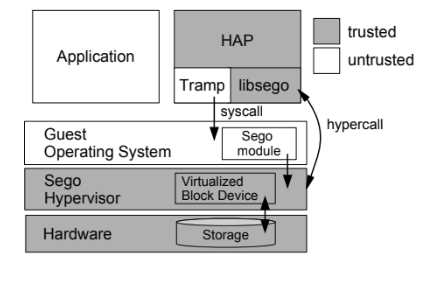
\includegraphics[width=0.6\linewidth]{sego_architecture}}%
	\caption{Sego Architecture Overview}
	\label{segoArchitecture}
\end{figure}

Sego is designed to execute trusted code in an \gls{hap}.
After booting the \gls{os}, the hypervisor starts the \gls{hap}, in a way that the \gls{hap} itself can verify its own initial code and data, similar to a \gls{tpm}.
Once running, the hypervisor ensures that the \gls{hap}’s registers and trusted address space are isolated from the \gls{os}. Everytime the \gls{hap} wants to perform a system call, it must inform
the hypervisor of its intent, so that the hypervisor can verify the \gls{os}'s activity. \gls{hap}s use a
small library called libsego as a way to handle system calls and get Sego services without having to change their code. Each \gls{hap} also contains an untrusted trampoline code, that
uses to interact with the \gls{os}. This protects its control-flow, since it uses this trampoline as issuer for system calls, therefore never compromising the \gls{hap} itself. Figure \ref{fig:segoArchitecture} shows well enough Sego’s overall design without going into too much dept, indicating which components are included in the \gls{tcb} and which are not.
Context switches are handled by the hypervisor, thus hiding any information about the \gls{hap} from the \gls{os}.

Sego does not guarantee \gls{os} availability. A compromised \gls{os} can simply shut down or refuse to schedule processes. However this is easily detected.



----------

			drawback of those approaches (inktag, virtghost...)
			and why aren't enough
			
-------------------------- END OF TO DO -----------------------------

% =======================
%  N E W   S E C T I O N        (2.2)
% =======================

\section{Hardware-Enabled TEE - Trusted Execution Environments}

A \gls{tee} is an abstraction provided by both software and hardware that guarantees isolated execution of specific programs in a machine, including the host \gls{os}, hypervisor or even system administrators, preventing them from leveraging their privileges. A \gls{tee} also provides integrity of applications running inside it, along with confidentiality of their assets.

The first attempts to implement a \gls{tee} on a cloud system consisted of combining a hypervisor with isolation properties and a \gls{tpm}. 

A \gls{tpm} \cite{tpmPaper} consists of a hardware chip, called microcontroller, that aims to create a trustable platform through encryption and authenticated boot, and make sure it remains trustworthy through remote attestation. 
It provides cryptographic functions that can't be modified, and a private key (Endorsment Key) that is unique to every \gls{tpm} made, working as an identifier for the \gls{tpm} itself.

However, \gls{tpm}s have several problems when applied to cloud systems, due to being designed with the intention to offer security to a single machine. It is not flexible enough to guarantee that anyone can get the encrypted data from a different node.
Thus, a distributed environment would not be the best kind of environment for a \gls{tpm} to work on.

The current best practice for protecting secrets in a cloud system uses \gls{hsm}s. 

\gls{hsm} \cite{hsmPaper} are physical components whose main function is to provide and store cryptographic keys used to encrypt/decrypt data inside a system. \gls{hsm}s can also perform cryptographic operations (e.g. encryption, hashing, etc.) as well as authenticate through verification of digital signatures and accelerate \gls{ssl} connections \cite{hsmThesis}, by relieving the servers from some of the workload caused by operations envolving cryptography. 

Thus, the system can protect critical secrets, such as cryptographic keys, and support a range of cryptographic functions.

With that in mind, new hardware-enabled solutions were developed to be more flexible and cloud friendly than the \gls{tpm}, or to incorporate the advantages of \gls{hsm} to the system. We'll dive into technologies like ARM TrustZone, Intel SGX, AMD-SEV, and others, in the following section.


% =======================
%  N E W   S E C T I O N        (2.3)
% =======================


\section{Hardware-Enabled TEE Solutions}


The idea of using hardware to provide trusted execution environments started appearing as a way to deal with piracy, with examples like TCPA \cite{tcpaPaper} and Microsoft's Palladium being the most known ones. By making use of hardware, it was possible to encrypt data (DVD's, for example) that could only be decrypted by a specific hardware, making it almost impossible to copy. 

Although this approaches were effective back in the day, both of them place their trust in the hardware, not trusting the \gls{os} entirely. 
Thus, since any application does not trust the \gls{os}, it does not trust the application to properly use its resources either. Therefore, some of the protection aspects of the \gls{os} must be moved into the hardware, as well as changing the interface between the \gls{os} and the application so it supports the hardware security features. 

\gls{xom}, described in the next subsection, was developed as a way to deal with these changes that were required to use this idea of trusted computing in a better way.

\subsection{XOM}

\gls{xom} \cite{xomPaper}, which stands for eXecute Only Memory, is a processor architecture that is able to provide copy protection and tamper-resistence functions, 
good for enabling code to run in untrusted platforms, deployment of trusted clients in distributed systems like banking transactions, online gaming and electronic voting, but also fundamental to deal with piracy back in the day it was published. 

The main idea is to only trust the processor to protect the code and data, thus not trusting the main memory nor any software, including the host \gls{os}.
However, this idea of only trusting hardware has some implications for \gls{os}es design. This happens due to the fact that sharing hardware resources between multiple users is a hard job, specially without trusting any software. It is usually easier to have this policies performed by the \gls{os}. Therefore, not trusting the software entirely can sometimes be a drawback.  

For \gls{xom} architecture to be used, it is required a specific \gls{os} (XOMOS). XOMOS runs on hardware that supports tamper-resistant software, and is adapted to manage hardware resources for applications that do not trust it.

\gls{xom} offers protection against attackers who may have physical access to the hardware itself, as well as main memory protection, if compromised. For it, the XOM processor encrypts the values in memory and stores the hash of those values in memory as well. It then only accepts encrypted values from memory if followed by a valid respective hash. 



\subsection{ARM TrustZone}
\label{ssec:armtz}

ARM TrustZone \cite{armTZPaper} are ARMs approach to offer a \gls{tee} where software can execute in a secured and trustable way, safe from the host machine, as well as its \gls{os} and/or hypervisor. 

To accomplish this, ARM processors implement two virtual processors backed by hardware access control, where the software stack can switch between two states: secure world (SW) and normal world (NW). 
The first one has higher priviledges than the second one, therefore it can access NWs copies of registers, but not the other way around. SW is also responsible of protecting running processes in the \gls{cpu}, while providing secured access to peripherals. 
Each world acts like a runtime environment and has its own set of resources. This resources can be partioned between the two worlds or just assigned to one of them, depending on the ARM chip specs.

For the context switch between worlds, ARM processors implement a secured mode called Secure Monitor, where there is a special register responsable of determine if the processor runs code in SW or NW. 

Most ARM processors also offer memory curtaining. This consists on the Secure Monitor allocating physical addresses of memory specifically to the SW, making this region of memory unaccessible to the rest of the system.

By default, the system boots always in SW so it can provision the runtime environment before any untrusted code start to run. It eventually transitions to NW where untrusted code can start to be executed. 

\subsection{AMD-SEV}
\label{ssec:amdsev}
AMD Secure Encrypted Virtualization (SEV) is the AMD approach to provide a \gls{tee}, integrated with virtualization. It is a technology focused primarily on cloud computing environments, specifically in public \gls{iaas}, as its main goal is to reduce trust from higher priviledged parties (\gls{vmm}s or \gls{os}), so that they can not influence the execution on the other "smaller" parties (\gls{vm}s). 

To achieve this, AMD grants encryption of memory through a technology called Secure Memory Encryption (SME), or through TransparentSME (TSME) if the system runs a legacy \gls{os} or hypervisor with no need for any software modifications.
After the data is encrypted, SEV integrates it with AMD virtualization architecture to support encrypted \gls{vm}s. By doing this, every \gls{vm} is now protected from his own hypervisor (\gls{vmm}), unabling its access to the decrypted data. Although uncapable of accessing the \gls{vm}, the \gls{vmm} is still responsible of controlling each \gls{vm}'s resources. \cite{amdPaper}

Thus, AMD provides confidentiality of data by removing trust from the \gls{vmm}, and creates an isolated environment for the \gls{vm} to run, where only the \gls{vm} and the processor can be trusted. However it does not provide integrity of data, allowing replaying attacks to take place, and has a considerably large \gls{tcb}, since the \gls{os} of each \gls{vm} is trusted. \cite{amdSEVPaper}

\subsection{Sanctum}
\label{ssec:sanctum}
The main objective of Sanctum \cite{sanctumPaper} is to offer strong isolation of software modules, altough following a different approach focused in avoiding unnecessary complexity, thus granting a simple security analysis.
To make this possible, Sanctum, which tipically runs in a RISC-V processor, combines minimal invasive hardware modifications with a trusted software security monitor that is receptive to analysis and does not perform cryptographic operations using keys. 

This minimality idea consists on reusing and slightly modifying existing well-understood mechanisms, while not modifiying \gls{cpu} building blocks, only adding hardware to the interfaces between blocks, causing Sanctum to be adaptable to many other processors besides RISC-V. 

Sanctum is a pratical approach that shows that a strong software isolation is achievable with a small set of minimally invasive hardware changes, causing reasonably low overhead. 
This approach provides strong security guarantees dealing with side-channel attacks, such as cache timing and passive address translation attacks.

\subsection{Intel-SGX}
\label{ssec:intelsgx}
Intel Software Security Guard Extensions (SGX) are a set of instructions built in Intel \gls{cpu}s, that allows programmers to create \gls{tee}s, by using enclaves. Enclaves are isolation containers that create a trusted environment where sensitive code can be stored and executed inside, ensuring integrity and confidentiality to it. By doing so, it reduces the \gls{tcb} in a way that most of the system software, apart from the enclaves and the \gls{cpu}, is considered not trusted.

Enclaves are mapped into private regions of memory, where only the \gls{cpu} has access to. Due to this restrictions, not even the most common system libraries can be accessed inside the enclave, since even the \gls{os} is not considered trusted. 

A system that encorporates \gls{sgx} under its architecture is divided in two: a trusted component being the enclave, and an untrusted component being the rest of the system. The untrusted one requests the launch of the enclave, where the \gls{cpu} then manages to allocate the enclave in a private region of memory, made available only to that particular enclave. This portion of memory is kept encrypted in volatile memory, being only decrypted by the \gls{cpu} if the responsible enclave requests it \cite{guiBorgesThesis}.

Altough isolation is the main objective of \gls{sgx}, it still allows a way for both  untrusted and trusted parties to communicate. This is made possible by the functions ECALL and OCALL. ECALLs are used for an untrusted component to call for trusted code in a secured way - the enclave copies the pointers to that specific code into a buffer, which is then made visible for the untrusted component, ensuring that the untrusted party can't know the real memory address inside the enclave. To communicate the other way around, the enclave calls for an OCALL, where the enclave is temporarily exited, executing then the unstrusted function needed. After that, the enclave is re-entered. OCALLS are mainly used by the enclave to access the network or to deal with I/O disk access.

% =======================
%  N E W   S E C T I O N        (2.4)
% =======================


\section{SGX-Enabled Frameworks and Shielded Applications}

The need for cloud computing is constantly growing in modern applications. 
It is a cost-effective and pratical solution to run large distributed applications, however the fact that it requires users to trust the cloud provider with their code and data creates some trust concerns for developers.

Although the usage of \gls{tee}s like \gls{sgx} aim to tackle this problem by running and storing sensitive data on a isolated environment, protecting that data from unauthorized access, \gls{sgx} itself has some limitations, and does offer this extra level of security at some costs for the systems. 

Hence, to deal with the \gls{sgx} limitations, some approaches were developed to be implemented on top of it, as a way to make systems more pratical by the integration of trusted computation. 
We will discuss those approaches in the next subsections.



\subsection{Shielded protected applications in untrusted Clouds}

As said previously, cloud computing is becoming more and more adopted in todays systems. 
Therefore, by being a such popular technology, it is a must that their users' data remains confidential. 
However, most of todays cloud systems are build using a classical hierarchical security model that only aims to protect the cloud providers' code from untrusted code (users' virtual machine), while doing nothing in terms of protecting the users' data. 
Hereupon, the users of a cloud platform must trust the provider software entirely, as well as the provider staff (i.e. system administrators or anyone with physical access to the hardware).

Several approaches were developed as a way to deal with this potential problem, by implementing the notion of shielded execution for applications running in the cloud. 

This concept consists on running server applications in the cloud inside of an isolated compartment. The cloud provider is limited to offering only raw resources (computing power, storage and networking) to the compartment, without being able to access any of the users data, except the one being transmitted over the network. 

Assuring a shielded execution of an application fundamentally means that both confidentiality and integrity of the data and code running are granted, and that if the application executes, it behaves just as it is expected. As for the provider, it retains control of the resources, and may protect itself from a malicious guest \cite{havenPaper}. 


\subsection{SCONE}

Container-based virtualization has become quite popular for offering better performance properties than the use of \gls{vm}s, however it offers weaker isolation guarantees, therefore less security. 
That is why we observe that containers usually execute network services (i.e. Redis). These are systems that don't need as much system calls as the other services, since they can do a lot via networking, thus keeping a small TCB for increased security.

SCONE \cite{sconePaper} is a mechanism for Linux containers that increases the confidentiality and integrity of services running inside them by making use of Intel-\gls{sgx}.

SCONE increases the security of the system while trying to keep the performance levels reasonable. 
It does it by: 
(1) keeping the size of the container's \gls{tcb} as small as possible, by linking a (small) library inside the enclave to a standard C library interface exposed to container processes. The system calls are executed outside the enclave, and networking is protected by \gls{tls}. 
(2) maximizes the time threads spend inside the enclave by supporting user-level threading and assynchronous system calls, thus allowing a thread outside the enclave to execute system calls without the need for enclave threads to exit.
This increases the performance since major performance losses are caused by enclave threads entering/exiting, due to the costs of encrypting/decrypting the data.



\subsection{Haven}

Haven is the first system to achieve shielded execution of unmodified legacy applications for a commodity \gls{os} (Windows) and hardware, achieving mutual distrust with the host software.

It leverages Intel-\gls{sgx} to protect against privileged code and physical attacks, but also against the challenge of executing unmodified legacy binaries while protecting them from an untrusted host.

Instead of shielding only specific parts of applications and data by placing them inside enclaves, Haven aims to protect entire unmodified applications, written without any knowledge of \gls{sgx}. 

However, executing entire chunks of legacy binary code inside a \gls{sgx} enclave pushes the limits of the \gls{sgx} itself, and while the code to be protected was written assuming that the \gls{os} executing the code would run it properly, this may not be the case, since the \gls{os} can be malicious. For this latest problem, the so called "Iago attack", Haven uses a library OS adapted from Drawbridge \cite{drawbridge}, running inside a \gls{sgx} enclave. 
By combining it with a remote attestation mechanism, Haven is able to guarantee to the user end-to-end security without the need of trusting the provider.

Although this approach may need a substantial \gls{tcb} size (LibOS quite large), all this code is inside the enclave, which makes it under users control. 

That's the main goal of Haven: give the user trust by granting confidentiality and integrity of their data when moving an application from a private area to a public cloud. 


\subsection{OpenSGX}

OpenSGX \cite{opensgx_paper} was developed as a way to help with the access to \gls{tee} software technologies, since these type of technologies were only available for a selected group of researchers. 
It was made available as an open source platform, and by providing \gls{tee} and \gls{os} emulation, it contributed a lot for expanding the possibility of research in this area, as well as promoting the development of SGX applications. 

OpenSGX emulates the hardware components of Intel-SGX and its ecosystem, including \gls{os} interfaces and user library, as a way to run enclave programs. To emulate Intel-\gls{sgx} at intruction-level, OpenSGX extended an open-source emulator, QEMU.
Its pratical properties result of six components working together: (1) Hardware emulation module: \gls{sgx} emulation, by providing \gls{sgx} instructions, data structures, \gls{epc} and its access protection, as well as \gls{sgx}' processor key; (2) \gls{os} emulation: since some \gls{sgx} instructions are priviledged (should be executed by the kernel), OpenSGX defines new system calls to perform \gls{sgx} operations, such as dynamic memory allocation and enclave provisioning; (3) Enclave loader: enclave must be properly loaded to \gls{epc}; (4) User library: provides a library (sgxlib) with a useful set of functions to be used inside and outside the enclave; (5) Debugging support; (6) Performance monitoring: allow users to collect performance statistics about enclave programs.

\begin{figure}[htbp]
	\centering
	{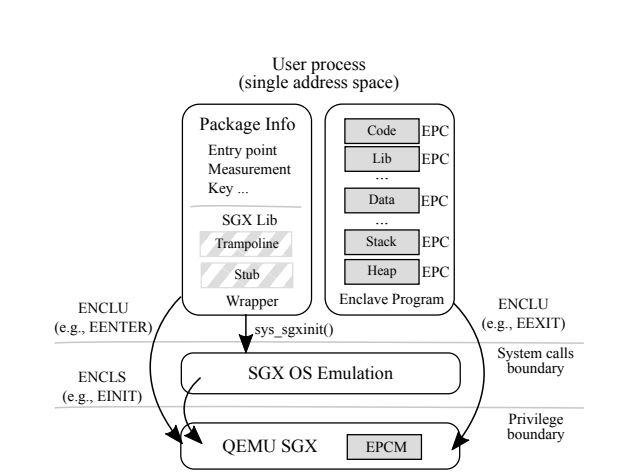
\includegraphics[width=0.6\linewidth]{opensgx_design}}%
	\caption{Overview design of OpenSGX framework and memory state of an active enclave program}
	\label{openSGXDesign}
\end{figure}

In Figure \ref{fig:openSGXDesign} we see an overall example of this framework, where a regular program (Wrapper) and a secured program (Enclave Program) both run as a single process in the same virtual address space. Due to the fact that Intel-\gls{sgx} uses privilege instructions to setup enclaves, the requests from the Wrapper program are handled by the OpenSGX set of system calls.

OpenSGX was proven capable of running non-trivial applications, as well as promoting the implementation and evaluation of new ideas. By being the first open-source framework to emulate a \gls{sgx} environment, it was shown to be fundamental to the growth of the \gls{tee} field.


\subsection{Panoply}

Panoply \cite{panoplyPaper} is a system that works as a bridge between \gls{sgx}-native abstractions and standard \gls{os} abstractions, required by most commodity Linux applications. 
It divides a system into multiple components, called micro-containers (or "micron"), and runs each one of them inside its own enclave. 
However, when microns communicate with each other, their communication goes through a channel under the \gls{os} control. Thus, Panoply design goals are focused on supporting \gls{os} abstractions with a low \gls{tcb}, while also securing inter-enclave communications.

Panoply's design consist on a set of runtime libraries (shim library included) and a build toolchain that helps developers to prepare microns.
With this, a programmer can assign annotations to functions as a way to specify which micron should execute a specific function. If not assigned any annotation, a function will be designated to a default micron, who shall execute it. Inter-micron flow integrity is also provided during this stage. 

Each micron is given a micron-id when it starts, which will be used for all further interactions with other microns. It will use this id as a way to assure that only authorized microns can send/receive messages.
To extend this inter-micron interaction security, Panoply also provides authenticated encryption of every message, makes use of unique sequence numbers, and acknoledgement messages are sent for every inter-enclave communication, thus protecting the containers from silent aborts, replaying, or tampering attacks.

Unlike many other \gls{sgx}-based frameworks, Panoply supports unlimited multi-threading and forking. Multi-threading in a way that, if a micron reaches its maximum concurrent thread limit, a new micron is launched and all shared memory operations are safely performed. Forking is achieved by replicating a parent micron's data and sending it to the child, over a secure communication. 


\subsection{VC3}
\label{ssec:vc3_mapreduce}

Verifiable Confidential Cloud Computing (VC3) \cite{vc3Paper} is a framework that achieves confidentiality and integrity of data, as well as verifiability of execution of code with good performance through MapReduce \cite{mapReduce} techniques. It uses Intel SGX processors as a building block and runs on unmodified Hadoop \cite{hadoop}.
In VC3 users implement MapReduce jobs, compile and encrypt them, thus obtaining a private enclave code E-. They then join it with a small portion of public code E+, that implements the protocols for key exchange and job execution.
Users then upload the resulting binary code to the cloud, where enclaves containing both E- and E+ are initialized by an untrusted framework F. 

\begin{figure}[htbp]
	\centering
	{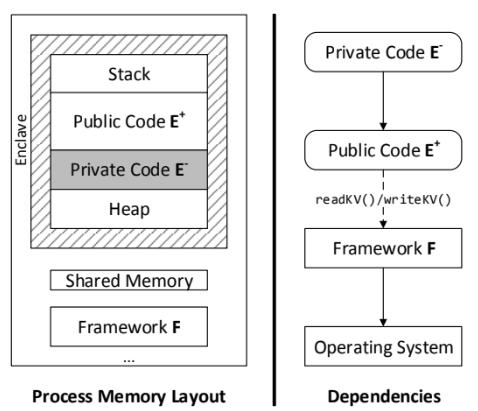
\includegraphics[width=0.6\linewidth]{vc3_design}}%
	\caption{VC3 memory design model on the left, component dependencies on the right}
\end{figure}

A MapReduce begins with a key exchange between the user and the E+ code running in the enclave. After this, E+ can proceed to decrypt E- and process the encrypted data. VC3 isolates this processing from the OS by keeping an interface between the E+ layer and the outside of the enclave. This interface consists of basically two functions: readKV() and writeKV(), for reading a key-value pair on Hadoop or write it, respectively. Also, the data inside of the enclave is passed to the outside, more specifically from E+ to the untrusted F, by using a virtual address space shared by both.
With VC3, both E- and the user data are always encrypted while in the cloud, except when processed by the trusted processor, while allowing Hadoop to manage the execution of VC3 jobs. Map and reduce nodes are seen as regular worker node to Hadoop, therefore Hadoop can provide its normal scheduling and fault-tolerance mechanisms, as well as load balancing. VC3 accomplishes this keeping Hadoop, the OS and the hypervisor out of the TCB.

\subsection{Protected Zookeeper}
\label{ssec:protected_zookeeper}

ZooKeeper \cite{zookeeper} is a replicated synchronization service for distributed systems with eventual consistency. However, ZooKeeper does not guarantee privacy of data stored inside of it by default.

Protected ZooKeeper \cite{protectedZooKeeper} is an approach that eliminates this privacy concerns, by placing an aditional layer between the client and the ZooKeeper, refered as ZooKeeper Privacy Proxy (ZPP). ZPP is a layer responsible for the encryption of all sensitive information, during a communication between a client and the ZooKeeper. 
Clients communicate with the proxy via a SSL connection, where the packets are encrypted by an individual session key. Here, ZPP acts like a normal ZooKeeper replica to the client. 
After receiving the packets from the client, ZPP extracts the sensitive data, encrypts it with a mechanism that allows the data to be decrypted by the proxy later on, and forwards the encrypted packet to a ZooKeeper replica where it can be stored with integrity ensured.

ZPP runs inside a TEE, located in the cloud, allowing it to store encryption keys and process plaintext data safely. As a result, even if the attacker is the cloud provider itself, the integrity of the data will still be granted since the attacker won't be able to access or alter anything running inside the TEE.

ZPP also retains all original ZooKeeper functionality, and does not affect ZooKeeper's internal behaviour. Therefore adapting existing ZooKeeper applications to this concept of ZPP it's easily done.

This approach allows applications in the cloud to use ZooKeeper without privacy concerns at the cost of a small decrease of throughput.
\subsection{Ryoan}
\label{ssec:ryoan_sandboxing}

Ryoan \cite{ryoanPaper} consists on a distributed sandbox that allows users to protect the execution of their data. This is achieved with the help of Intel SGX \cite{intelSGX} \cite{sgxPaper} enclaves, creating sandbox instances that protect data from untrusted software while also preventing leaks of data, which is a weakness of enclaves caused by side channel attacks.
Ryoan does not include any priviledged software (e.g. OS and hypervisor) in it's TCB, while trusting only the hardware (SGX enclave) to assure secrecy and integrity of the data.

It's main goal is to prevent leakage of secret data. This is done by preventing modules from sending sensitive data over their communications if outside the system boundaries, as well as eliminating stores to unprotected memory and system calls, made possible by the use of a trusted sandbox Native Client (NaCl). 

\begin{figure}[htbp]
	\centering
	{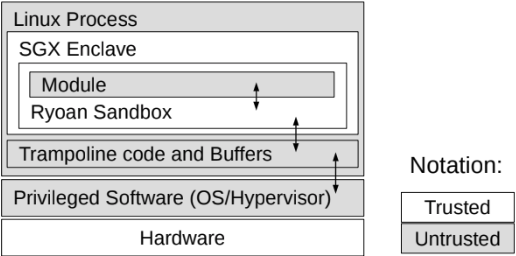
\includegraphics[width=0.6\linewidth]{ryoan_design}}%
	\caption{Instance of Ryoan running on a single machine}
\end{figure}

Ryoan's approach consists on confining the untrusted application in a NaCl, responsable of controlling system calls, I/O channels and data sizes. This NaCl sandbox is implemented inside the enclave, and can communicate with other instances of the NaCl, forming a distributed sandbox between users and different service providers. Inside the sandbox, the untrusted application can execute safely on secret data. The NaCl sandbox uses a load time code to ensure that the module can not do anything it shouldn't, thus violating the sandbox. To handle faults, exceptions or errors inside the NaCl sandbox, Ryoan uses an unprotected trampoline code, that can enter the enclave and read the information about the fault so it can handle it.
\subsection{Opaque}
\label{ssec:opaque}

Opaque \cite{opaquePaper} is a distributed data analytics platform that guarantee encryption, secure computation and integrity to a wide range of queries. Therefore, instead of being implemented in the application layer or the execution layer as this kind of security approaches usually are, Opaque is implemented in the query optimization layer. 

It is implemented with minimal modifications on Spark SQL, and uses Intel SGX technology as a way to grant confidentiality and integrity of the data. 
However, the use of enclaves can still be threatened by access pattern leakage that can occur at memory-level, when a malicious OS infers information about encrypted data just by monitoring memory page accesses, and at network-level, when network traffic reveals information about encrypted data.

Opaque hides access patterns in the system by using distributed oblivious relational operators and optimizes these by implementing new query planning techniques. It can be executed in three modes

\begin{itemize}
	\item encryption mode: provides data encryption and authentication, while granting correct execution.
	\item oblivious mode: provides oblivious execution, protecting against access pattern leakage.
	\item oblivious pad mode: extends the oblivious mode by adding prevention of size leakage.
\end{itemize}

Opaque is an approach that is able to grant oblivious execution 3 times faster than other specialized oblivious protocols.

\subsection{Graphene-SGX}
\label{ssec:grapheneSGX}

The usage of Intel SGX, and similar technologies, have proven to add a great sense of privacy to the storage and execution of data in applications. However this tecnologies impose restrictions (e.g., disallowing system calls inside the enclave) that require the applications to be changed so they can benefit from this extra layer of security. 

Graphene-SGX \cite{graphenePaper} came to help circunvent those restrictions, while still assure security to the data. It is a library OS that aims to reproduce system calls, respecting security concerns, so that unmodified applications can use them to keep executing normally without interacting directly with the OS or hypervisor. 

By using a library OS, the system is expected to lose performance and, since a new layer of software was added, to increase the size of the TCB. 
Although these assumptions are true, they are quite often exagerated. Graphene-SGX's performance goes from matching a Linux process to less than 2x in most executions of single-processes.
Graphene-SGX has also shown some great results comparing it to other similar approaches that use shim layers, such as SCONE \cite{sconePaper} and Panoply \cite{panoplyPaper}, where it shows to be performancewise similar to SCONE and faster 5-10 percent than Panoply, while adding 54k lines of code to the TCB compairing to SCONE's 97k and Panoply 20k.

Graphene's main goal is to run unmodified applications on SGX quickly. Thus, whilst the size of the TCB is not the smallest compairing to the other approaches, developers can reduce the TCB as needed as a way to reach a more optimal solution. 

Graphene-SGX also supports application partitioning, enabling it to run small pieces of one application in multiple enclaves. This can be useful, for instance, to applications with different privilege levels while still increasing the security of the application.
\subsection{Other approaches}
%todo

-------------------------- TO DO -----------------------------


Need any intro or just go straight to the subsections?

-------------------------- END OF TO DO -----------------------------


\subsubsection{SGX-Enabled Network Protocols and Services}
%todo

The increased need for security seen nowadays caused network related technologies to also become popular, from security protocols (TLS) to anonymous browsers (Tor), leading to a lot of effort by the community to make viable approaches to tackle network security problems. 
Hardware approaches capable of providing \gls{tee}s (e.g. Intel-\gls{sgx}) have recently been used to make some contributions to deal with modern network security concerns as a way to, for example, solve policy privacy issues in inter-domain routing, thus protecting ISPs policies.

In \cite{torSGXPaper} it’s shown that leveraging hardware protection of TEEs can grant benefits, such as simplify the overall design of the application, as well as securely introduce in-network functionality into TLS sessions. The same paper also presents a possible approach to reach security and privacy on a network level, by building a prototype on top of OpenSGX, that shows that SGX-enabled applications have modest performance losses compared to one with no SGX support, while significantly improving it’s security and privacy.

Also at the networking security level, the usage of Network Function Virtualization (NFV) architecture by applications nowadays imply the creation of internal state as a way to allow complex cross-packet and cross-flow analysis. 
These states contain sensitive information, like IP addresses, user details and cached content (e.g. profile pictures), therefore should be a priority to ensure their protection from potential threats.
To tackle this vulnerability, S-NFV \cite{sNFVPaper} has proven to be a valid approach, by providing a secure framework for NFV applications, securing NFV states by using Intel-SGX.

S-NFV divides the NFV application in two: S-NFV enclave and S-NFV host. The enclave is responsible to store the states and state processing code, while the host deals with the rest.

In \cite{sNFVPaper} by implementing the S-NFV approach with Snort \cite{snortPaper} on top of OpenSGX was
concluded that this SGX-enabled approach results in bigger overheads (aprox. 11x for
gets and 9x for sets) than an SGX-disabled Snort application, at the cost of extra security.


\subsubsection{Trusted Cloud-Based System Administration}
%todo
The use of cloud platforms lead to a significant increase of security and privacy risks. Thus, cloud services are now higly dependent on trusting its administrators, as well as their good behaviour. Since this is not always the case, it has become a must to protect the users from potencial cloud system administration threats. 
To tackle this problem, some solutions have been proposed with the help of trusted computing technology. However, their focus have been conducted on Infrastructure-as-a-Service (IaaS) environments, which are simpler to maintain than in PaaS and SaaS approaches.

\cite{sgxCloudThesis} proposes a solution that addresses trustworthy and security in PaaS and SaaS environments while preserving essential system administration functions by leveraging Intel-\gls{sgx}. By making use of \gls{sgx}, it provides an environment for cloud customers to review the security conditions of cloud nodes, more specifically those that run their applications and handle their data.

The main idea behind this approach is to allow the administrative staff necessary privileges according to escalation policies enforced for different roles, instead of never granting full administrative privileges on the computing nodes.

The administrative roles for cloud nodes are divided into four or five independent roles, depending if it's a SaaS or PaaS environment, each with their own permissions. Each role works under supervision of internal or external auditors. The internal auditors being the ones hired by the provider, while the external are hired by customers, as a way to execute protocols decided by both in a trustable way. The solution both enables control of cloud trusted nodes operational states, designated to run customer's computations, as well as remote attestation of the boot sequence of PaaS or SaaS stacks. Finally, by including logging of changes in node's states, this solution is able to offer trustworthy in the execution of functions and protocols.

This approach was shown in \cite{sgxCloudThesis} to have minimal performance impact, as well low storage overheads, while being a compelling approach to be used to increase detail of management protocols and tools in cloud environments and data-centers.


\subsubsection{SGX-enabled Virtualization}
%todo

Has we already pointed out previously, Intel-\gls{sgx} has drawn much attention from the community in the last few years, which also made cloud providers to start implementing \gls{sgx} into their cloud systems (Microsoft's Azure confidential computing or IBM Cloud are examples of that). Also, new cloud programming frameworks have already been created with the ability to support \gls{sgx}. 

However, while most of the research on Intel-\gls{sgx} have been concentrated on its security and programmability properties, there are a lot of questions to answer about how the usage of \gls{sgx} affects the performance of a virtualized system. This is relevant since virtualization is the main building block of cloud computing.

In \cite{sgxVirtualizationPaper} an exaustive evaluation about the performance of \gls{sgx} on a virtualized system, concluding that:

(1) Hypervisors don't need to intercept every \gls{sgx} instruction to enable \gls{sgx} for being virtualized. Was concluded that there is only one indispensable \gls{sgx} function, ECREATE, which is responsable to virtualize \gls{sgx} launch control.

As a result, gls{sgx} on \gls{vm}s is considered to have an acceptable overhead.

(2)  \gls{sgx} overhead on \gls{vm}s when running memory-heavy benchmarks consists mainly of address translation when using nested paging. If instead it uses shadow paging, the overhead becomes insignificant. 
\cite{sgxVirtualizationPaper} shows that this can be optimized by using shadow paging for \gls{epc} to reduce translation overhead, and nested paging for general usage.

(3) On the contrary, when running benchmarks involving many context switches (e.g., HTTP benchmarks), shadow paging performs worse than nested paging.

(4) The use of \gls{sgx} causes a heavy drop in performance switching between application and enclave, whether it's using virtualization or not. This drop causes server applications using \gls{sgx} to be affected.
\cite{sgxVirtualizationPaper} specifies that this can be addressed by using mechanisms (e.g. HotCalls \cite{hotcallsPaper}) that work as a fast call interface between the aplication and enclave code. This interfaces reduce the overhead of ecalls and ocalls, helping the porting of applications to \gls{sgx}.

(5) Swapping \gls{epc} pages is really expensive, and this also applies for all systems using \gls{sgx}. 
Upon the start, \gls{sgx} measures the contents of the enclave, thus triggering enclave swapping if enclave's memory size is larger than the available \gls{epc} size. 
This was shown in \cite{sgxVirtualizationPaper} to be optimizable by minimizing enclave's size, thus reducing swapping and consequently increasing enclave performance.
Virtualization causes an additional overhead, which increases based on the number of threads running inside the enclave.

Finally, \cite{sgxVirtualizationPaper} proposes an automatic selection of an appropriate memory virtualization technique, by dynamically detecting the characteristics of a given workload to identify whether it is suitable with nested or shadow paging.


\subsubsection{SGX-Enabled Linux Containers}
%todo
Lately, container solutions such as Linux Containers (LXC) and Docker have proved to be compelling alternatives to virtualization in cloud computing systems, due to the fact that they need less computing resources, allowing more deployments per physical machine to take place, as well as reducing infrastructure costs. However, some concerns have been raised since containers share a common \gls{os} kernel, therefore any vulnerability of the kernel would put all the other containers on the system in danger.

While various solutions including Haven, Graphene-SGX, SCONE, Panoply have been proposed to secure applications and containers in the cloud environment by using Intel-\gls{sgx}, these approaches still generate some concerns, like the need to expand the TCB and enclave size, limited support for key features like remote attestation, and ignore hardware constraints on \gls{epc} size (instead of relying on \gls{epc} page swapping, which lead to serious performance losses). 
This issues are the result of a still incomplete infrastructure, from the \gls{os} to the application layer. 

In \cite{lxcsgxPaper} these exact concerns are addressed by introducing a platform for Linux Containers (LXC) that leverage Intel-\gls{sgx} in the cloud environment, called lxcsgx. 
This lxcsgx platform offers an infrastructure that supports: (1) Remote attestation; (2) \gls{epc} memory control for containers to prevent malicious overuse of resources; (3) Software \gls{tpm} that can easily allow legacy applications to use \gls{sgx}; (4) GCC plugin to assist with the partitioning of applications, thus reducing the \gls{tcb}.

Lxcsgx was proven in \cite{lxcsgxPaper} to offer the lowest overhead to the overall system when compared to the previously spoken solutions, while also addressing potential issues these could have. 


\subsubsection{SGX-Enabled Searchable Encryption}
%todo

Processing and storing data in cloud environments is still considered too risky by many. To deal with this, systems started to support \gls{tee}s as a way to provide trust to their users, making sure all their data remains private. 
However, working with encrypted data is not always as easy as it sounds, since software-based approaches made specifically for search encrypted information still lack some properties, good performance being one of the main ones. Well known approaches like Fully Homomorphic Encryption (FHE), though they offer a good extra security properties, are not pratical in large distributed systems. As for hardware-based existing approaches, they proved not to scale well due to hardware limitations, as well as depending in a large \gls{tcb}, which can become susceptible to threats.

CryptDB \cite{cryptDBPaper} is a database system capable of processing SQL queries over encrypted data. It is an approach that supports order-preserving encryption for efficient search, which lead to a low performance overhead due to the use of internal index structures, and also allowing range queries on ciphertexts to happen the same way as if the data was in plaintext. However, some research can be seen in \cite{naveedPaper} about this particular type of encryption, showing that it is possible to recover the original plaintexts, thus making systems like this incapable of providing enough security guarantees to the data.

As a result, new approaches like HardIDX started to become more popular, for providing security properties by supporting the use of trusted execution techniques, while offering decent levels of performance.

HardIDX \cite{hardIDXPaper} is a hardware approach that provides the possibility of searching over encrypted data, leveraging Intel-\gls{sgx}. It implements only a small core of operations, in particular searches (on a single value or value ranges), in the \gls{tee}.
This approach uses B+-tree as the structure to organize all data, which is found in many \gls{dbms}s.

Unlike previous hardware-based approaches, HardIDX implements a small size \gls{tcb} and memory footprint in the \gls{tee}, thus exposing a small atack surface, as well as granting good performance results while executing complex searches on large chunks of data, all this while being able to scale the system to large indexes, as proved in \cite{hardIDXPaper}. 



\subsubsection{ShieldStore}
%todo
The increasing research on trusted computation technologies, in particular \gls{tee}s like \gls{sgx} made possible for cloud users to run their applications safely in potentially malicious systems. One of the most used type of applications in these cloud systems are key-value stores, like Redis \cite{redisWebsite} and memcached \cite{memcachedWebsite}. These type of data stores are used in many systems nowadays due to their architecture offering fast access to data, by maintaining data in main memory, as well as granting durability by writing the data to persistent storage.  Due to the importance of these type of systems in todays systems stack, there is a special interest in allowing them to be protected by trusted technology. However, one of the critical limitations of \gls{sgx} is the size of the \gls{epc}, which represents its protected memory region. 

To circumvent this memory restriction, a in-memory key-value store designed to leverage \gls{sgx}, ShieldStore \cite{shieldStorePaper}, was presented. ShieldStore provides fast execution of queries over large data, by maintaining the majority of the data structures outside enclave memory region, hence contributing to overcome \gls{sgx} memory limitations.

ShieldStore runs inside the enclave to protect encryption keys, remote attestation, and to perform all the logic necessary to the Key-Value Store execution.

ShieldStore design starts by remote attesting the server-side, verifying \gls{sgx} support of the processor, the code and other critical memory state of an enclave. Then, using Intel-\gls{sgx} libraries, the client and the server exchange keys so that a secure channel between both parties is created. The client then send a request, to which the server deciphers and verifies, and thus accessing the Key-Value Store for the desired data. To note that the client does not access the server's ciphertexts neither needs to know the key the server used to encrypt the values. The server then decrypts the stored data, and encrypts it again with the session key previously decided when establishing the secure channel with the client, and a reply is sent to the client.    

This is an approach capable of minimizing the unnecessary memory encryption overhead of paging, and also eliminate \gls{epc} page faults, which are the main factors impacting the performance of these kind of encrypted data storage systems. Also, ally to the optimization of the index structures, that enabled them for fast access and protection of keys and values, ShieldStore is proven to be an efficient, reliable Key-Value store capable of leveraging \gls{sgx} advantages.


\subsubsection{EnclaveDB}
EnclaveDB \cite{enclavedbPaper} is an approach to deal also with the need to protect data, both in the storage process and the processing of that data when accessing it. It offers confidentiality and integrity of queries and data, by working alongside Intel-\gls{sgx} in order to handle all the sensitive data (queries, tables, indexes) inside enclave memory, thus keeping the data safe in cases where the database administrator is malicious, when the \gls{os} or hypervisor is compromised, and even when running the database in an untrusted host. 

EnclaveDB's design is divided in two modules: trusted, running inside the enclave, and untrusted. The trusted compartment hosts a query processing engine, a transaction manager, pre-compiled stored procedures and a trusted kernel responsible for sealing and remote attestation. As for the untrusted module, it is responsible to run all the other components of the database system. 

This approach fundamentally provides a database system with a SQL interface with security guarantees, while dealing with low overhead. Also, by depending on a smaller \gls{tcb} than any other conventional database server, the security provided increases considerably, making EnclaveDB a valid approach to work as a secured database system.




\section{Summary and Discussion}
%todo
-------------------------- TO DO -----------------------------

ShieldStore vs EnclaveDB

Graphene

Dissertation Approach


-------------------------- END OF TO DO -----------------------------




\subsection{Discussion}
\label{ssec:sgx_frameworks_discussion}

Haven [15] showed
that a library OS could run unmodified applications on
SGX,

thin “shim” layers, like SCONE [14] and Panoply [49] wrap 
an API layer such as the system call table.


--------


SGX frameworks and applications.

VC3 [45]
runs MapReduce jobs in SGX enclaves.

Bren-
ner et al. [17] run cluster services in ZooKeeper in an
enclave, and transparently encrypt data in transit be-
tween enclaves.

Ryoan [22] sandboxes a piece of un-
trusted code in the enclave to process secret data while
preventing the loaded code from leaking secret data.

Opaque [57] uses an SGX-protected layer on the Spark
framework to generate oblivious relational operators that
hide the access patterns of distributed queries.

The \novathesis\ class can be customized with the options listed below.




